\documentclass{article}
%% Language and font encodings
\usepackage[french]{babel}
\selectlanguage{french}
\usepackage[T1]{fontenc}

%% Sets page size and margins
\usepackage[a4paper,top=3cm,bottom=2cm,left=3cm,right=3cm,marginparwidth=1.75cm]{geometry}

%% Useful packages
\usepackage{amsmath}
\usepackage{graphicx}
\usepackage[colorinlistoftodos]{todonotes}
\usepackage[colorlinks=true, allcolors=blue] {hyperref}
\usepackage[utf8]{inputenc}
\title{Manuel d'utilisation du jeu akiba.}
\author{Marin Dorange Launey\\
		L1 info Gr 4B\\
        21601861}
        
\begin{document}
\maketitle

\begin{figure}[!h]
\centerline{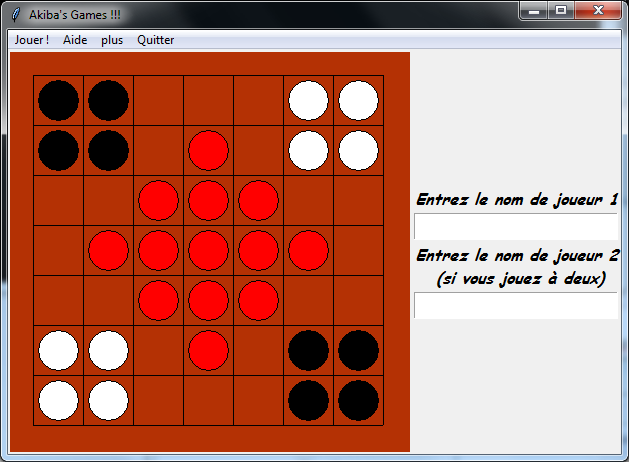
\includegraphics[width=0.6\textwidth]{images/Akiba.png}}
\vspace{1cm}
\caption{}
\end{figure}

\newpage{}
\tableofcontents{}

\newpage{}

\section{Introduction du jeu d'Akiba.}
Le jeu d'akiba est un jeu de société creé en 1994 par Serge Cahu,il est aussiconnu sous le nom de Traboulet ou encore Kuba.Il s'addresse aux enfants comme aux adultes.Malgré les rumeurs ce jeu est trés différents dans sa maniere de jouer par rapport au célèbre jeu de société Abalone.Par exempe,dans ce jeu, au contraire de Abalone, il ne faut pas un certains nombre de boules pour pousser les boules adverse. Toutes fois si vous souhaité acheté ce jeu de société en france vous ne pourrait pas car l'editeur de jeu Fun Connection ne le commercialise plus à cause de ces rumers de soit disant plagiat du jeu Abalone.

\section{Les régles du jeu.}

Tout d'abord ce jeu ce joue à deux sur un plateau de 7 case par 7 case contenant 8 boules noir,8 boule blanche et 13 boules rouges.
\begin{figure}[!h]
\centerline{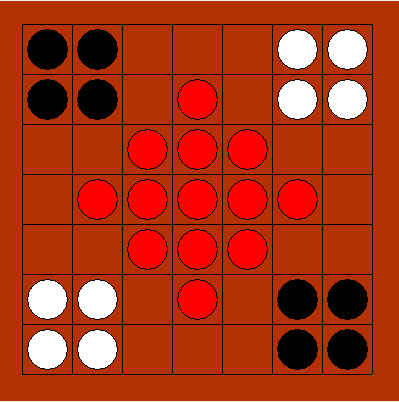
\includegraphics[width=0.6\textwidth]{images/plateau_akiba.png}}
\vspace{0.5cm}
\caption{}
\end{figure}
\newpage{}
Le but de ce jeu est soit de sortir les 8 boules adverse ou 7 boules rouges.
Toute fois quelque régles regisent ce jeu.En effet il est interdit de sortir ces propre boules,nous n'avons pas le droit de déplacer une boules si une quelconque boules ce trouves derriére celle-ci.Par exemple dans la figure 2,sachant que les boules noir numéro 1,3,4 sont accolé au bord, la boule noir 2 ne peut être jouer car avant elle il'y a soit la boule numéro 1 soit la boule numéro 4.Par contre on peut jouer les boules 1,3,4 car ,les bord étant considérait comme des espaces vide, il y'a un espace pour "placer sont pouce" avant la boule.
\begin{figure}[!h]
\centerline{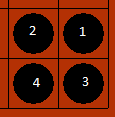
\includegraphics[width=0.2\textwidth]{images/Coup_interdit.png}}
\vspace{0.5cm}
\caption{}
\end{figure}

Enfin, si le joueur adverse deplace nos boules,au tour suivant nous n'avons pas le droit d'effectuer un mouvement inverse pour remettre nos boules.


\section{Comment jouer sur notre jeu ?}
Tout d'abord,sur notre page d'acceuil nous pouvons voir 3 partie:

\vspace{0.5cm}
\begin{figure}[!h]
\centerline{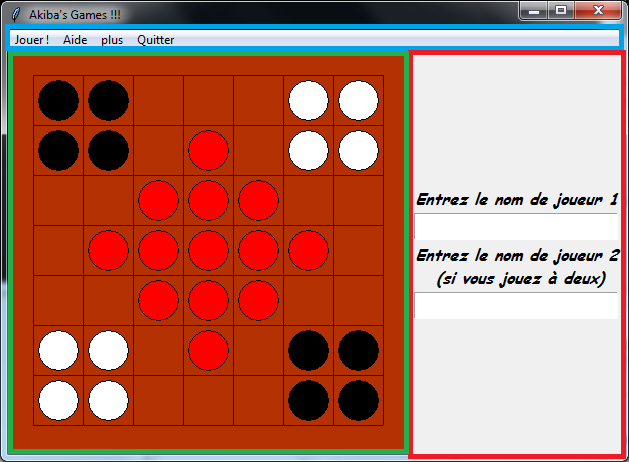
\includegraphics[width=0.6\textwidth]{images/fenetre_debut.png}}
\vspace{0.5cm}
\caption{}
\end{figure}

\begin{itemize}
\item Le plateau de jeu d'akiba,en position initiale.(cadre vert figure 1)
\item un menu déroulant,contenant les bouttons pour commencer une partie ou afficher des informations.(cadre bleu figure 1)
\item une zone pour prendre notre nom, et afficher des informations par la suite.(cadre rouge figure 1 )
\end{itemize}
\vspace{0.25cm}
Ensuite notre jeu peut se jouer de deux maniéres différentes.:
\begin{itemize}
\item Soit l'on joue contre une personne.
\item Soit l'on joue contre une IA.
\end{itemize}
\vspace{0.5cm}


\subsection{Jouer à deux.}
Pour Jouer à deux vous n'avez qu'a remplir vos noms à droite,puis allez dans l'onglet jouer et cliquez sur jouez à deux.La partie démarre alors automatiquement.L'affichage à droite change alors:
\begin{figure}[!h]
\centerline{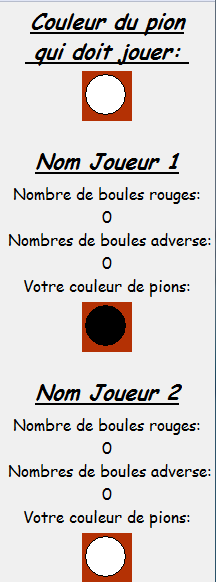
\includegraphics[width=0.3\textwidth]{images/Affichage_Jouer_deux.png}}
\vspace{0.5cm}
\caption{}
\end{figure}
\newpage{}
\subsubsection{Début de la partie.} On peut ainsi voir sur cette affichage(figure 4).
\begin{itemize}
\item tout d'abord la couleur du pions qui doit jouer.
\item Ensuite s'affiche le nom du joueur 1 ainsi que ses scores et une boules montrant la couleur de ses boules. 
\item Enfin le joueur 2 à le même affichage que joueur 1 juste en dessous.
\end{itemize}
\subsubsection{Une fois la partie lancée}
Une fois que la partie à débuté il faut, pour déplacer ses pions faire un clic gauche sur la boule (ou sur la premiére boules d'une rangée) que l'on veut déplacer puis refaire un clic gauche dans la direction du mouvement souhaité.


\subsection{Jouer Seul contre l'IA.}
Pour jouer seul face à l'ordinateur, il faut remplir sont nom droite dans la premiére case. Puis ensuite allez dans l'onglet jouer! et cliquez sur jouer seul. La partie démarre alors automatiquement est l'affichage change ainsi:

\begin{figure}[!h]
\centerline{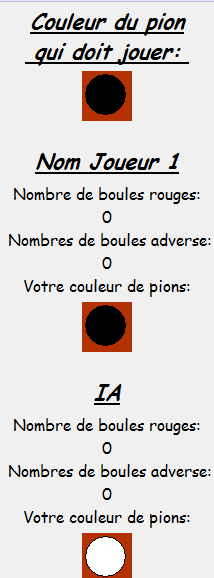
\includegraphics[width=0.3\textwidth]{images/Affichage_Jouer_seul.png}}
\vspace{0.5cm}
\caption{}
\end{figure}

\newpage{}

\subsubsection{Début de la partie.} On peut ainsi voir sur cette affichage (figure 4).
\begin{itemize}
\item tout d'abord la couleur du pions qui doit jouer.
\item Ensuite s'affiche le nom du joueur 1 ainsi que ses scores et une boules montrant la couleur de ses boules. 
\item Enfin suivant l'affichage dont dispose le joueur 1 on peut suivre les scores de l'IA.
\end{itemize}
\subsubsection{Une fois la partie lancée}
Une fois que la partie à débuté il faut, pour déplacer ses pions faire un clic gauche sur la boule (ou sur la premiére boules d'une rangée) que l'on veut déplacer puis refaire un clic gauche dans la direction du mouvement souhaité.Quand à l'IA elle jouera automatiquement.


\section{Fin d'une partie.}
Une fois le score réglementaire pour gagner atteind, une pop-up s'afficher à l'écran: 

\begin{figure}[!h]
\centerline{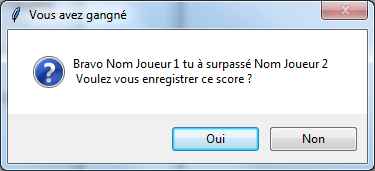
\includegraphics[width=0.6\textwidth]{images/pop-up_fin_partie.png}}
\vspace{0.5cm}
\caption{}
\end{figure}

\subsection{Enregistrer une partie.}
Si vous voulez enregistrer le score que vous venez de faire face à un autre joueur ou face à l'ordinateur cliquez sur "oui" sinon cliquez sur "non" (figure 6).
\subsection{Revoir ses ancient scores}
Pour revoir ses anciens scores il suffit d'allez dans l'onglet "plus" du menu et de choisir de rechercher toute ses parties ou celles contre des Joueurs (sans d'IA comme deuxiéme joueur). Une fenêtre apparait alors:

\begin{figure}[!h]
\centerline{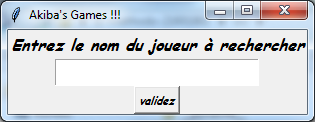
\includegraphics[width=0.6\textwidth]{images/Saisie_Nom.png}}
\vspace{0.5cm}
\caption{}
\end{figure}

\newpage{}

Il faut alors rentrez le pseudo/nom rentrez lors d'une partie précédente pour voir s'afficher les résultats:

\begin{figure}[!h]
\centerline{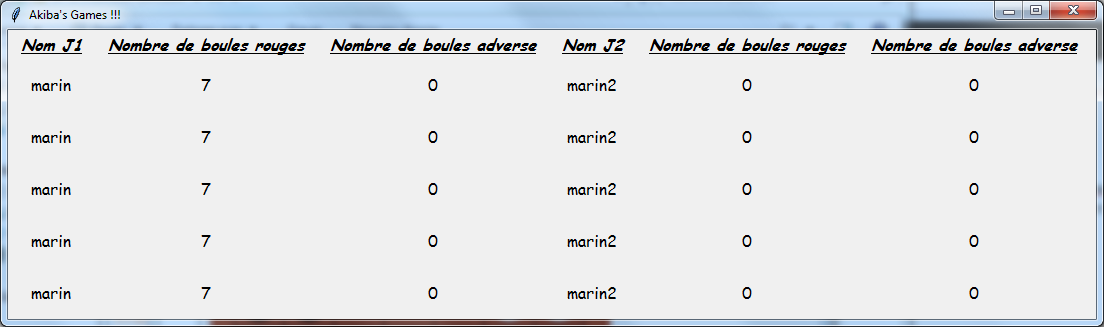
\includegraphics[width=0.6\textwidth]{images/Affichage_score.png}}
\vspace{0.5cm}
\caption{}
\end{figure}

\subsection{Effacer les scores.}
Enfin vous pouvez effacer tout les scores réaliser en allant dans l'onglet "plus" du menu et en cliquant sur "Réinitialiser les scores (les effacer)".
\end{document}























